\documentclass[nojss]{jss}

\usepackage{float}
\usepackage{graphicx}
\usepackage{amsmath}
\usepackage{natbib}

%%%%%%%%%%%%%%%%%%%%%%%
% BEGIN Custom Commands %
%%%%%%%%%%%%%%%%%%%%%%%

\newcommand{\Sref}[1]{Section~\ref{#1}}  
\newcommand{\argmin}{\operatornamewithlimits{arg\,min\ }}  
\newcommand{\argmax}{\operatornamewithlimits{arg\,max\ }}  
\newcommand{\mean}{\text{mean}}    
\newtheorem{claim}{Claim}

%%%%%%%%%%%%%%%%%%%%%%%
% END Custom Commands %
%%%%%%%%%%%%%%%%%%%%%%%

%%%%%%%%%%%%%%%%%%%%%%%
% BEGIN TikZ Commands %
%%%%%%%%%%%%%%%%%%%%%%%

\usepackage{tikz}
\usetikzlibrary{shapes, arrows}
\usepackage{amsmath}
\usepackage{xspace}
\newcommand{\A}{\ensuremath{\mathcal{A}}\xspace}
\newcommand{\B}{\ensuremath{\mathcal{B}}\xspace}
\newcommand\pa[1]{\ensuremath{\left(#1\right)}}

%%%%%%%%%%%%%%%%%%%%%
% END TikZ Commands %
%%%%%%%%%%%%%%%%%%%%%

%%%%%%%%%%%%%%%%%%%%%%%%%%%%%%
%% declarations for jss.cls %%
%%%%%%%%%%%%%%%%%%%%%%%%%%%%%%

%% almost as usual
\author{Gary King\\Harvard University \And 
        Christopher Lucas\\Harvard University \And 
        Richard Nielsen\\MIT}
\title{\pkg{MatchingFrontier}: \proglang{R} Package for Computing the Matching Frontier\thanks{The current release of \pkg{MatchingFrontier} is in active development and will continue to grow over the coming months. Comments and suggestions are greatly appreciated.}}

%% for pretty printing and a nice hypersummary also set:
\Plainauthor{Gary King, Christopher Lucas, Richard Nielsen} %% comma-separated
\Plaintitle{MatchingFrontier: R Package for Computing the Matching Frontier} %% without formatting
\Shorttitle{\pkg{MatchingFrontier}} %%  short title (if necessary)

%% an abstract and keywords
\Abstract{ \pkg{MatchingFrontier} is an \proglang{R} package that
  implements the methods described in \citet{kingND} for optimizing
  both balance and sample size in matching methods for causal
  inference. \pkg{MatchingFrontier} supports the computation of
  frontiers for both continuous and discrete metrics and also provides
  functions for visualizing the frontier and exporting matched data
  sets for further analysis.}

\Keywords{\proglang{R}, matching, frontier, Mahalanobis, L1}
\Plainkeywords{R, matching, frontier, Mahalanobis, L1} %% without formatting
\Address{
  Gary King\\
  Department of Government\\
  Harvard University\\
  1737 Cambridge St, Cambridge, MA, USA\\
  E-mail: \href{mailto:king@harvard.edu}{king@harvard.edu}\\
  URL: \href{http://gking.harvard.edu/}{http://gking.harvard.edu/}\\

  Christopher Lucas\\
  Department of Government\\
  Harvard University\\
  1737 Cambridge St, Cambridge, MA, USA\\
  E-mail: \href{mailto:clucas@fas.harvard.edu}{clucas@fas.harvard.edu}\\
  URL: \href{http://christopherlucas.org/}{christopherlucas.org}\\

  Richard Nielsen\\
  Department of Political Science\\
  Massachusetts Institute of Technology\\
  77 Massachusetts Avenue, Cambridge, MA, USA\\
  E-mail: \href{mailto:rnielsen@mit.edu}{rnielsen@mit.edu}\\
  URL: \href{http://www.mit.edu/~rnielsen/index.htm}{http://www.mit.edu/~rnielsen/index.htm}

}
%% It is also possible to add a telephone and fax number
%% before the e-mail in the following format:
%% Telephone: +43/512/507-7103
%% Fax: +43/512/507-2851

%% for those who use Sweave please include the following line (with % symbols):
%% need no \usepackage{Sweave.sty}

%% end of declarations %%%%%%%%%%%%%%%%%%%%%%%%%%%%%%%%%%%%%%%%%%%%%%%

\begin{document}

%% include your article here, just as usual
%% Note that you should use the \pkg{}, \proglang{} and \code{} commands.

\section[Introduction]{Introduction}

Matching methods have become extremely popular amongst researchers
working with observational data, especially when used as a
nonparametric preprocessing step to reduce model dependence
\citep{ho2007,ho2009}. But despite this popularily, existing matching
approaches leave researchers with two fundamental tensions. First,
they are designed to maximize one metric (such as propensity score or
Mahalanobis distance) but are judged against another for which they
were not designed (such as $L1$ or differences in means). Second, they
lack a principled solution to revealing the implicit bias-variance
trade off: matching methods need to optimize with respect to both
imbalance (between the treated and control groups) and the number of
observations pruned, but existing approaches optimize with respect to
only one; users then either ignore the second or tweak it without a
formal stopping rule.

\pkg{MatchingFrontier} resolves both tensions by consolidating
previous techniques into a single, optimal, and flexible approach. The
software calculates the matching solution with maximum balance for
each possible sample size $(N, N-1, N-2,...)$ and returns each
solution, the whole of which constitute the \emph{frontier}, from
which the user can easily choose one, several, or all subsamples with
which to conduct the final analysis, given their own choice of
imbalance metric and quantity of interest. \pkg{MatchingFrontier}
solves the joint optimization problem in one run, automatically,
without manual tweaking, and without iteration.  Although for each
subset size $k$, there exist a huge number of unique subsets $N
\choose k$, \pkg{MatchingFrontier} includes specially designed and
extremely fast algorithms that give the optimal answer, usually in a
few minutes or less.

\section[What MatchingFrontier Does]{General Framework}\label{sec:framework}

Matching methods are designed to reduce imbalance in data by
selectively pruning observations, which in turn reduces model
dependence \citep{king2006,imai2008,iacus2011a,ho2007}. However,
pruning reduces sample size and therefore may increase variance in the
eventual estimates. Users of matching are then confronted with the
perennial bias-variance trade-off. Perhaps surprisingly, existing
approaches to matching do not conduct the implied joint optimization
of bias and variance. Rather, they improve one dimension of the
optimization and leave the second to the user. Such an approach is
time consuming and rarely yields the optimal solution.

\citet{kingND} proposes a solution to this joint optimization, which
is implemented in \pkg{MatchingFrontier}. Discrete and continuous
metrics are defined and algorithms are provided for both continuous
and discrete metrics, thus rendering the method agnostic to the
metric. We point users of \pkg{MatchingFrontier} to \citet{kingND} for
algorithmic details and theoretical proofs. In this section, we
provide definitions of the metrics so that users can choose
appropriately when using \code{makeFrontier()}.

For discrete metrics, we follow \citep{iacus2011b} and use the
difference between the multivariate histograms of the treated and
control groups. Formally, let $f_{\ell_1\cdots \ell_k}$ be the
relative empirical frequency of treated units in a bin with
coordinates on each of the $X$ variables as $\ell_1\cdots \ell_k$ so
that $f_{\ell_1\cdots \ell_k}=n_{T_{\ell_1\cdots \ell_k}}/n_T$ where
$n_{T_{\ell_1\cdots \ell_k}}$ is the number of treated units in
stratum $\ell_1\cdots \ell_k$ and $n_T$ is the number of treated units
in all strata. We define $g_{\ell_1\cdots \ell_k}$ similarly among
control units. Then:
\begin{equation}\label{eq:L1} 
  L_1(H) =\frac{1}{2} \sum_{(\ell_1
    \cdots \ell_k) \in H} |f_{\ell_1\cdots \ell_k} - g_{\ell_1\cdots
    \ell_k}| 
\end{equation} 

For continuous metrics, we define the Average Mahalanobis Imbalance
(AMI). Though easily generalized to all continuous measures of
distance, we choose Mahalanobis distance. AMI is the distance between
each unit $i$ and the closest unit in the opposite group, averaged
over all units: $D=\mean_i [D(X_i,X_{j(i)})]$, where the closest unit
in the opposite group is
$X_{j(i)}=\argmin_{X_j|j\in\{1-T_i\}}[D(X_i,X_j)]$ and $\{1-T_i\}$ is
the set of units in the (treatment or control) group that does not
contain $i$. \pkg{MatchingFrontier} defaults to AMI but can just as
easily be used with $L_1$.

Of note is that these metrics presume a dichotomous treatment.  Given
recent advances in matching with continuous treatments \citep{iacusND,
  ratkovicND}, we encourage researchers to consider generalizing our
algorithms (and therefore, metrics) to continuous treatment regimes.

\section[Getting Started]{Getting Started}

\pkg{MatchingFrontier} is written in the \proglang{R} language
\citep{r2012} and is currently hosted on Github and CRAN. CRAN hosts
the latest stable release. You can install the current development
release of \pkg{MatchingFrontier} with the \pkg{devtools} package
\citep{wickham2013}, as follows.

\begin{Schunk}
\begin{Sinput}
> library(devtools) 
> install_github('ChristopherLucas/MatchingFrontier/package')
\end{Sinput}
\end{Schunk}

Alternatively, you can install the development version of
\pkg{MatchingFrontier} from a *nix command line as follows.

\begin{Schunk}
\begin{Soutput}
 $ curl -OL https://github.com/ChristopherLucas/MatchingFrontier/archive/master.zip
 $ unzip master.zip
 $ cd MatchingFrontier-master
 $ R CMD INSTALL package
\end{Soutput}
\end{Schunk}

\section[A User's Guide]{A User's Guide}

The typical \pkg{MatchingFrontier} workflow is displayed in
Figure~\ref{fig:workflow}. Note that in nearly all cases, users first
proceed through the two-step process of computing the frontier and
then estimating quantities of interest across it. After these steps
are completed, the results can be used to visually summarize the full
frontier or to closely inspect a particular point on it.  Next, we
illustrate this workflow with the LaLonde data
\citep{lalonde1986,dehejia1999}, which is included in
\pkg{MatchingFrontier}.


\begin{figure}[H]
\centering
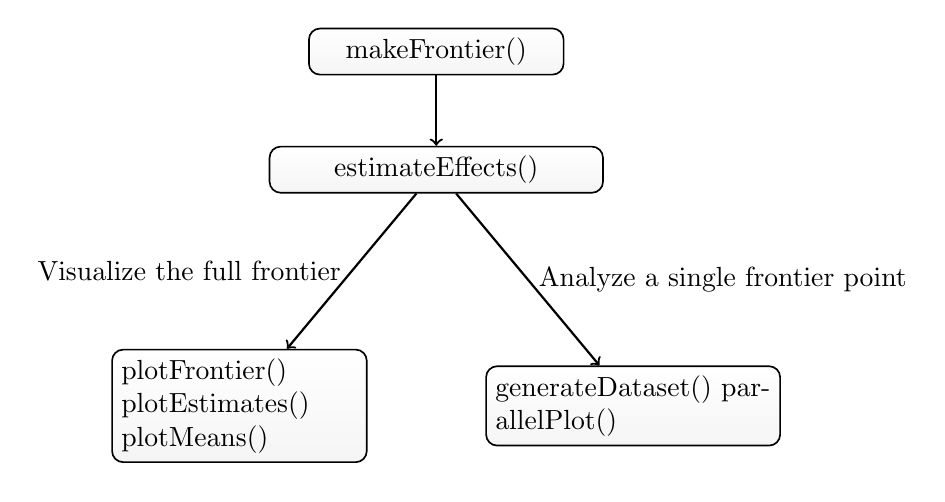
\begin{tikzpicture}[
    grow = down,
    ->,thick,
    sibling distance=6cm,
    level 1/.style={sibling distance=6cm, level distance = 1.5cm},
    level 2/.style={sibling distance=5cm, level distance = 3cm}, 
    %%%%%%%%%%%%%%%%%%%%%%%%%%%%%%%%%%%%%%
    make/.style={rectangle, rounded corners, shade, top color=white,
    bottom color=white!80!black!20, draw=black, 
    semithick,text width = 3cm,align = center},
    %%%%%%%%%%%%%%%%%%%%%%%%%%%%%%%%%%%%%%
    estimate/.style={rectangle, rounded corners, shade, top color=white,
    bottom color=white!80!black!20, draw=black, 
    semithick,text width = 4cm,align = center},
    %%%%%%%%%%%%%%%%%%%%%%%%%%%%%%%%%%%%%%
    export/.style={rectangle, rounded corners, shade, top color=white,
    bottom color=white!80!black!20, draw=black, 
    semithick,text width = 3.5cm,align = left},
    %%%%%%%%%%%%%%%%%%%%%%%%%%%%%%%%%%%%%%
    plotting/.style={rectangle, rounded corners, shade, top color=white,
    bottom color=white!80!black!20, draw=black, 
    semithick,text width = 3cm,align = left},
    ]
    \tikzstyle{every node}=[circle,draw]
    \node[make]{\code{makeFrontier()}}
        child { 
            node[estimate] {\code{estimateEffects()}}
            child { node[plotting] {\code{plotFrontier()} 
                                    \code{plotEstimates()} 
                                    \code{plotMeans()}} 
              edge from parent node[left,draw=none]{Visualize the full frontier} 
            }
            child { node[export]{\code{generateDataset()} 
                                 \code{parallelPlot()}} 
              edge from parent node[right,draw=none]{Analyze a single frontier point}}
        }
          ;
\end{tikzpicture}
\caption{A typical \pkg{MatchingFrontier}
  workflow. \code{makeFrontier()} is used to construct the frontier,
  then \code{estimateEffects()} is used to estimate quantities of
  interest for each point on the frontier, after which the user may
  proceed to visualize the full frontier or to inspect individual
  points on it.}\label{fig:workflow}
\end{figure}

\subsection{LaLonde Example}

For the running example in this paper, we use a randomly selected
subset of the ``LaLonde'' data \citep{lalonde1986,
  dehejia1999}\footnote{For a complete description of the data, type
  \code{?lalonde} after loading \pkg{MatchingFrontier}.}. The LaLonde
data is commonly used to assess matching methods and refers to the
combination of data from an experimental intervention containing 185
treated units (the National Supported Work Demonstration) with
observational data. By combining the experimental data with
observational data, methods can be compared to the underlying
experimental benchmark. We follow \citet{lalonde1986} and combine the
results of the experimental intervention with the Current Population
Survey. In \citet{kingND}, we analyze the Lalonde data plus the full
data set from the Current Population Study. In this paper, we keep
the 185 treated units and randomly selected 1,000 controls from the 
full data. This allows users to quickly replicate and adapt the
code presented in this paper. See \citet{kingND} for a serious
substantive analysis. 

The LaLonde data contains a treatment indicator ``treat'' (an
indicator for assigment to a jobs training program), an outcome
measure ``re78'' (income in 1978), and a number of controls (potential
confounders) that we will match on during the illustration. The
controls are as follows.

\begin{itemize}
  \item[\textbf{age}:] subject age at time of intervention
  \item[\textbf{education}:] years of education
  \item[\textbf{black}:] a race indicator for identification as black
  \item[\textbf{hispanic}:] an ethnicity indicator for identification as hispanic
  \item[\textbf{married}:] an indicator for whether or not the subject is married
  \item[\textbf{nodegree}:] an indicator for whether or not the subject has a college degree
  \item[\textbf{re74}:] income in 1974
  \item[\textbf{re75}:] income in 1975
\end{itemize}

\subsection{Computing the Frontier}

The user must first create the frontier. To do so, use the
\code{makeFrontier()} function, which will calculate the optimal
subsample at every point on the frontier. By default,
\code{makeFrontier()} calculates the frontier with the Average
Mahalanobis Imbalance. However, as we demonstrate,
\pkg{MatchingFrontier} works just as easily with $L_1$ difference.

First, calculate the Mahalanobis frontier for the LaLonde
data.

\begin{Schunk}
\begin{Sinput}
> # Load the package and the data
> library(MatchingFrontier)
> data('lalonde')
> # Create a vector of column names to indicate which variables we 
> # want to match on. We will match on everything except the treatment
> # and the outcome.
> match.on <- colnames(lalonde)[!(colnames(lalonde) %in% c('re78', 'treat'))]
> match.on # Print variables in match.on
\end{Sinput}
\begin{Soutput}
[1] "age"       "education" "black"     "hispanic"  "married"   "nodegree" 
[7] "re74"      "re75"     
\end{Soutput}
\begin{Sinput}
> # Make the mahalanobis frontier
> mahal.frontier <- makeFrontier(dataset = lalonde, 
+                             treatment = 'treat', 
+                             outcome = 're78', 
+                             match.on = match.on)
\end{Sinput}
\begin{Soutput}
Calculating Mahalanobis distances...
Calculating theoretical frontier...
Calculating information for plotting the frontier...
\end{Soutput}
\begin{Sinput}
> mahal.frontier
\end{Sinput}
\begin{Soutput}
An imbalance frontier with 997 points.
\end{Soutput}
\end{Schunk}

As shown above, \code{match.on} is a vector holding the variable names
that the user wishes to match on. Because \code{re78} is
the outcome and \code{treat} is the treatment, we exclude those
variable names from the vector.

By default, \code{makeFrontier()} calculates the frontier for the
Average Mahalanobis Imbalance, as defined in
Section~\ref{sec:framework}.  The default quantity of interest is the
\emph{feasible sample average treatment effect on the treated} or
FSATT \citep{kingND}, for which weights are calculated and returned to the
user. 

To instead calculate the $L_1$ frontier, simply
provide optional ``metric'', ``QOI'', and ``ratio'' arguments, as
follows.\footnote{For technical explanations of these arguments, we
  point users to \citet{kingND}.}

\begin{Schunk}
\begin{Sinput}
> # Make the L1 frontier
> L1.frontier <- makeFrontier(dataset = lalonde, 
+                             treatment = 'treat', 
+                             outcome = 're78', 
+                             match.on = match.on,
+                             QOI = 'SATT',
+                             metric = 'L1',
+                             ratio = 'fixed')
\end{Sinput}
\begin{Soutput}
Calculating L1 binnings...
Calculating L1 frontier... This may take a few minutes...
\end{Soutput}
\begin{Sinput}
> L1.frontier
\end{Sinput}
\begin{Soutput}
An imbalance frontier with 976 points.
\end{Soutput}
\end{Schunk}

Next, we will use the results computed above to estimate causal
effects along the frontier.

\subsection{Estimating Effects}

Continuing with the Lalonde example, we will estimate the effects
along the frontier with the \code{estimateEffects()} function, which
takes the output from \code{makeFrontier()} to estimate the effect of
the treatment along all values of the frontier. With the Lalonde
example, the code is as follows.

\begin{Schunk}
\begin{Sinput}
> # Estimate effects for the mahalanobis frontier
> mahal.estimates <- estimateEffects(mahal.frontier, 're78 ~ treat')
> # Estimate effects for the L1 frontier
> L1.estimates <- estimateEffects(L1.frontier, 're78 ~ treat',
+                                 model.dependence.points = 100)
\end{Sinput}
\end{Schunk}

\code{estimateEffects()} takes two arguments. The first argument is
the output from \code{makeFrontier()} and the second is the formula
passed to the \code{lm()} function. \code{estimateEffects} stores the
estimates and the 95\% confidence interval for each point it
estimates.

Alternatively, we could also condition on the variables that we are
matching on (stored in \code{match.on}) by specifying a different
formula, as follows.

\begin{Schunk}
\begin{Sinput}
> # Estimate effects for the mahalanobis frontier
> mahal.estimates.controls <- 
+     estimateEffects(mahal.frontier, paste('re78 ~ treat +', 
+                                           paste(match.on, collapse = ' + ')))
> # Estimate effects for the L1 frontier
> L1.estimates.controls <- 
+     estimateEffects(L1.frontier, paste('re78 ~ treat +', 
+                                        paste(match.on, collapse = ' + ')))
\end{Sinput}
\end{Schunk}

We've now estimated effects along the full frontier for AMI with and
without controls and for $L_1$ with and without controls. Next, we
will visually inspect the full frontier.

\subsection{Plotting the Frontier}

We can plot the frontier and the estimates with the plotting
functions, as follows. Note that for the sake of brevity, we will only
do so with the $L1$ frontier (no controls). However, to plot the other
three frontiers calculated in the previous section, simply pass the
corresponding objects to the plotting functions, as the syntax is the
same.

First, we will plot the frontier, where the $y$-axis is $L1$ and the
$x$-axis is the number of observations pruned. This is displayed in
Figure~\ref{fig:mahal_frontier_plain} next to the code that generated
it.

\begin{minipage}{0.45\textwidth}
\begin{Schunk}
\begin{Sinput}
> # Plot frontier
> plotFrontier(L1.frontier)
\end{Sinput}
\end{Schunk}
\end{minipage}
\begin{minipage}{0.5\textwidth}
\begin{figure}[H]
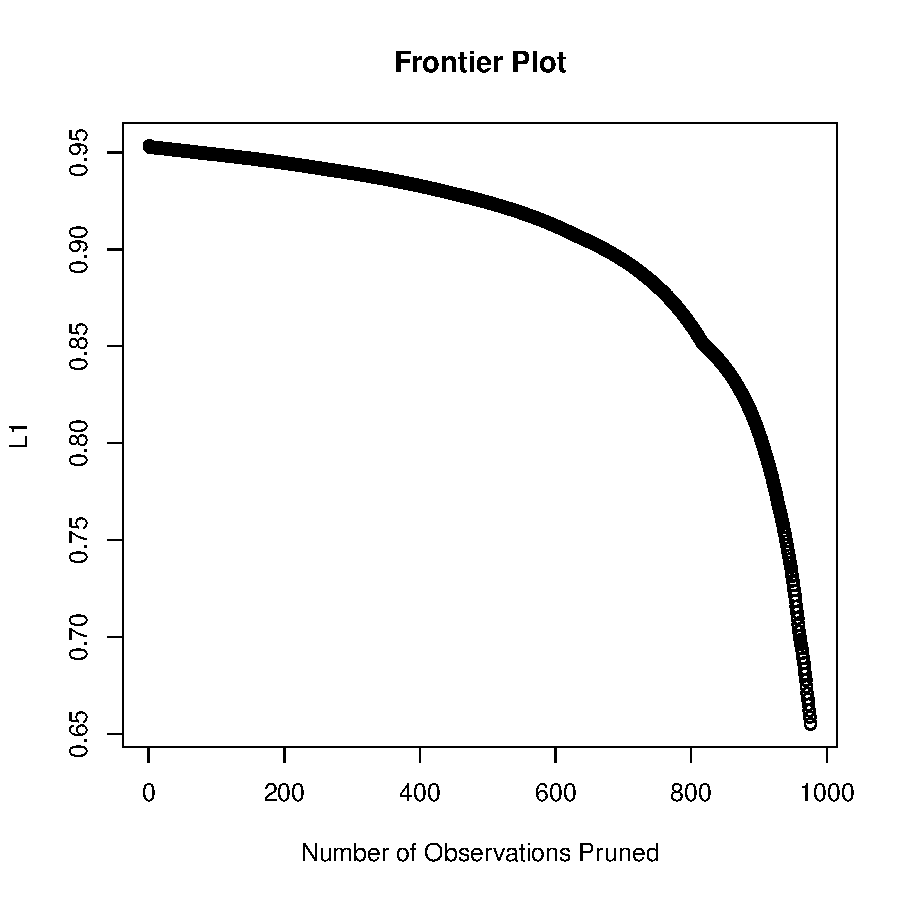
\includegraphics{Using_MatchingFrontier-mahal_frontier_plain.pdf}
\caption{\label{fig:mahal_frontier_plain} The L1 frontier without optional arguments}
\end{figure}
\end{minipage} \hfill

However, Figure~\ref{fig:mahal_frontier_plain} is not especially
attractive.  The font is too small and the dots constituting the
frontier run into each other and create an ugly, fat line. All of the
plotting functions in \pkg{MatchingFrontier} use \proglang{R}'s
ellipsis feature to permit access to the base plotting
functionality. Figure~\ref{fig:mahal_frontier_pretty} shows an
example, along with the corresponding code.


\begin{minipage}{0.45\textwidth}
\begin{Schunk}
\begin{Sinput}
> # Plot frontier
> plotFrontier(L1.frontier,
+              cex.lab = 1.4,
+              cex.axis = 1.4,
+              type = 'l',
+              panel.first = 
+                 grid(NULL, 
+                      NULL, 
+                      lwd = 2)
+              )
\end{Sinput}
\end{Schunk}
\end{minipage}
\begin{minipage}{0.5\textwidth}
\begin{figure}[H]
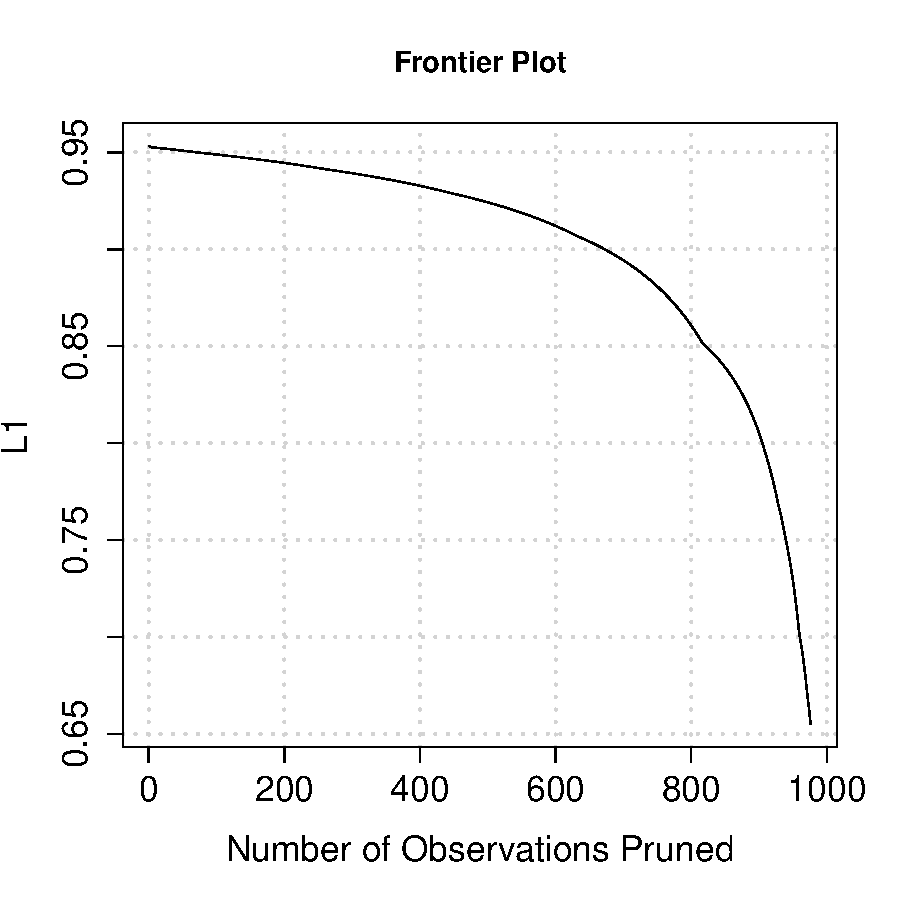
\includegraphics{Using_MatchingFrontier-mahal_frontier_pretty.pdf}
\caption{\label{fig:mahal_frontier_pretty} The $L1$ frontier with optional arguments}
\end{figure}
\end{minipage} \hfill

\subsection{Plotting Estimates}

Next, we can plot estimates along the frontier. As in the previous
section, we will use the $L1$ frontier without controls. To do so,
we'll use the results from \code{makeFrontier()} and
\code{frontierEst()}. Figure~\ref{fig:mahal_frontier_est} displays these
results.

\begin{minipage}{0.45\textwidth}
\begin{Schunk}
\begin{Sinput}
> # Plot estimates
> plotEstimates(L1.estimates, 
+               ylim = 
+                   c(-10000, 3000),
+               cex.lab = 1.4,
+               cex.axis = 1.4,
+               type = 'l',
+               panel.first = 
+                  grid(NULL,
+                       NULL,
+                       lwd = 2,
+                       )
+               )
\end{Sinput}
\end{Schunk}
\end{minipage}
\begin{minipage}{0.5\textwidth}
\begin{figure}[H]
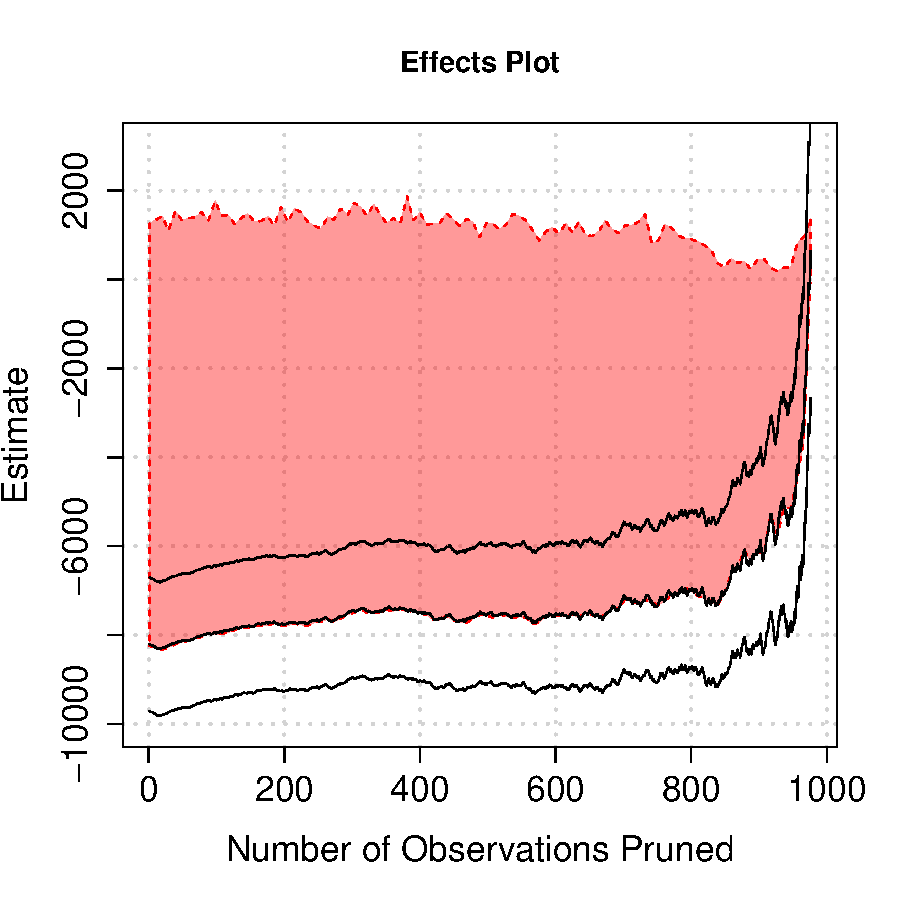
\includegraphics{Using_MatchingFrontier-mahal_frontier_est.pdf}
\caption{\label{fig:mahal_frontier_est} Estimates across the $L1$ frontier.}
\end{figure}
\end{minipage} \hfill

\subsection{Inspect a Single Point on the Frontier}

Lastly, users may wish to export a data set on the frontier for
additional analysis. To do so, users are likely to rely on
\code{parallelPlot()} and \code{generateDataset()}. Parellel plot
allows the user to visually inspect multiple dimensions of a data set
and requires only the output of \code{makeFrontier()}. For
illustration, we will create a parallel plot that displays 
the treated and control values on `age', `re74', `re75', and
`black' for the point on the frontier where 785 observations
have been dropped. We will color treated units \textcolor{blue}{blue}
and control units \textcolor{gray}{gray}.

\begin{minipage}{0.45\textwidth}
\begin{Schunk}
\begin{Sinput}
> # Make parallel plot
> parallelPlot(L1.frontier,
+              N = 400,
+              variables = c('age',
+              're74',
+              're75',
+              'black'),
+              treated.col = 'blue',
+              control.col = 'gray'
+              )
\end{Sinput}
\end{Schunk}
\end{minipage}
\begin{minipage}{0.5\textwidth}
\begin{figure}[H]
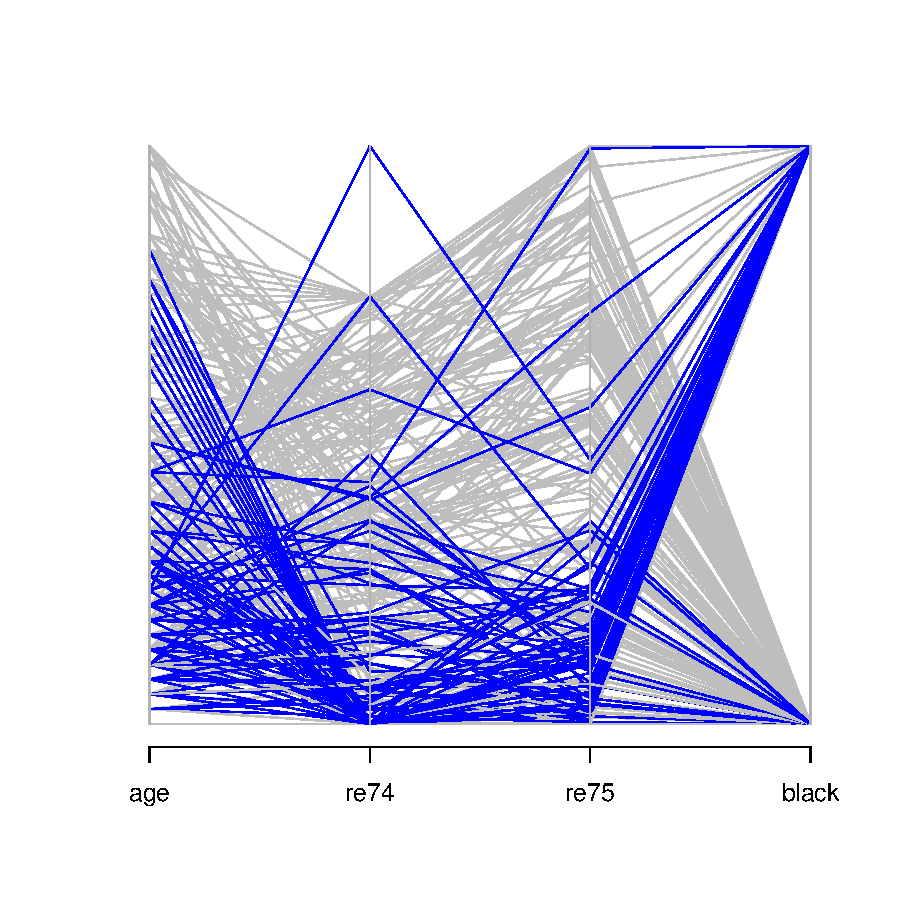
\includegraphics{Using_MatchingFrontier-mahal_parplot.pdf}
\caption{\label{fig:mahal_parplot} Parallel plot for pruning 785 observations.}
\end{figure}
\end{minipage} \hfill

Figure \ref{fig:mahal_parplot} makes obvious the fact that there are
many more control than treated units and that the sample still
contains a large number of controls that are not good matches for
treated units, at least on these dimensions. Though this implies that
perhaps we might move even further down the frontier, for
illustration, let's now export this data set, using
\code{generateDataset()} as follows.

\begin{Schunk}
\begin{Sinput}
> n <- 400 # Identify the point from which to select the data
> matched.data <- generateDataset(L1.frontier, N = n)
\end{Sinput}
\end{Schunk}

If the estimand is variable ratio, as it is by default, the exported
data set will include the appropriate weights necessary for estimating
the FSATT. We can now run a few simple regressions, controlling for
the variables we matched on, using the matched data.\footnote{Table
  generated by \pkg{Stargazer} \citep{hlavac14}.}


% Table created by stargazer v.5.1 by Marek Hlavac, Harvard University. E-mail: hlavac at fas.harvard.edu
% Date and time: Thu, Jan 22, 2015 - 07:58:15 PM
\begin{table}[!htbp] \centering 
  \caption{} 
  \label{} 
\begin{tabular}{@{\extracolsep{5pt}}lcc} 
\\[-1.8ex]\hline 
\hline \\[-1.8ex] 
 & \multicolumn{2}{c}{\textit{Dependent variable:}} \\ 
\cline{2-3} 
\\[-1.8ex] & re78 & re78 \\ 
\\[-1.8ex] & (1) & (2)\\ 
\hline \\[-1.8ex] 
 treat & $-$6,984.022$^{***}$ & 1,011.661 \\ 
  & (886.364) & (1,120.759) \\ 
  & & \\ 
 age &  & $-$14.088 \\ 
  &  & (44.293) \\ 
  & & \\ 
 education &  & 306.848 \\ 
  &  & (213.445) \\ 
  & & \\ 
 black &  & $-$550.212 \\ 
  &  & (1,091.106) \\ 
  & & \\ 
 hispanic &  & $-$1,508.171 \\ 
  &  & (1,447.458) \\ 
  & & \\ 
 married &  & 441.041 \\ 
  &  & (974.394) \\ 
  & & \\ 
 nodegree &  & $-$489.522 \\ 
  &  & (1,165.794) \\ 
  & & \\ 
 re74 &  & 0.115 \\ 
  &  & (0.093) \\ 
  & & \\ 
 re75 &  & 0.566$^{***}$ \\ 
  &  & (0.098) \\ 
  & & \\ 
 Constant & 13,333.170$^{***}$ & 2,234.911 \\ 
  & (602.793) & (3,304.559) \\ 
  & & \\ 
\hline \\[-1.8ex] 
Observations & 400 & 400 \\ 
R$^{2}$ & 0.135 & 0.402 \\ 
Adjusted R$^{2}$ & 0.133 & 0.388 \\ 
Residual Std. Error & 8,838.675 (df = 398) & 7,425.526 (df = 390) \\ 
F Statistic & 62.085$^{***}$ (df = 1; 398) & 29.096$^{***}$ (df = 9; 390) \\ 
\hline 
\hline \\[-1.8ex] 
\textit{Note:}  & \multicolumn{2}{r}{$^{*}$p$<$0.1; $^{**}$p$<$0.05; $^{***}$p$<$0.01} \\ 
\end{tabular} 
\end{table} 
\section[Conclusion]{Conclusion}

We demonstrated how to use the new \proglang{R} software package
\pkg{MatchingFrontier} for causal inference with observational data. With the
LaLonde data, users were shown how to compute the balance-sample size frontier,
calculate estimates along it, and visualize and inspect the results. 

\pagebreak
\bibliography{bibliography}
\end{document}
